\chapter{Orchestrated Objective Reduction (Orch-OR) Theory}
\label{ch:orch-or}

\begin{nontechnical}
\textbf{Orch-OR is a controversial theory claiming consciousness comes from quantum physics happening in tiny tubes inside brain cells---like your thoughts are quantum computers running in microscopic scaffolding!}

\textbf{The wild idea}: - \textbf{Normal view}: Brain = electrical
signals between neurons = consciousness - \textbf{Orch-OR view}: Brain =
quantum superpositions in microtubules = consciousness - \textbf{Why
controversial}: Most scientists think it\textquotesingle s impossible
(brain too warm/wet for quantum effects)

\textbf{The two scientists}:

\textbf{1. Roger Penrose} (Nobel Prize-winning physicist): -
``Consciousness can\textquotesingle t be explained by normal computing''
- ``Quantum mechanics must collapse in an objective way
(gravity-related)'' - ``This creates conscious moments''

\textbf{2. Stuart Hameroff} (anesthesiologist): - ``Microtubules
(protein tubes in neurons) are quantum computers'' - ``Anesthesia works
by disrupting quantum effects in microtubules'' - ``This explains why
diverse drugs all cause unconsciousness''

\textbf{Simple analogy - Orchestra}: - \textbf{Neurons}: Like musicians
in orchestra (play notes) - \textbf{Microtubules}: Like the
conductor\textquotesingle s baton oscillations (quantum superpositions)
- \textbf{Orch-OR}: Baton collapses \$\textbackslash rightarrow\$
orchestra plays note \$\textbackslash rightarrow\$ conscious moment! -
Happens \textasciitilde40 times/second \$\textbackslash rightarrow\$
stream of consciousness

\textbf{What are microtubules?} - Tiny hollow tubes made of proteins
(tubulin) - In every cell (not just neurons) - Normally: Act as cell
skeleton, transport highways - Orch-OR claim: Also quantum computers for
consciousness!

\textbf{The big problem - ``Too warm, too wet''}: - Quantum effects
usually need: Cold (near absolute zero), isolated, vacuum - Brain is:
37\$\^{}\textbackslash circ\$C, wet, chaotic, full of molecules -
\textbf{Objection}: ``Quantum coherence would die in 10\^{}-13
seconds-\/-\/-way too fast!'' - \textbf{Response}: ``Quantum biology
shows nature is cleverer-\/-\/-see photosynthesis, bird navigation''

\textbf{Evidence FOR Orch-OR}: - \textbf{THz resonances found}:
Microtubules vibrate at specific frequencies (lab experiments) -
\textbf{Anesthetics bind to tubulin}: Explains why they cause
unconsciousness - \textbf{Quantum biology exists}: Photosynthesis, bird
magnetoreception use quantum effects - \textbf{Meyer-Overton rule}:
Anesthetic potency correlates with microtubule binding

\textbf{Evidence AGAINST Orch-OR}: - \textbf{Decoherence calculations}:
Quantum states should die too fast - \textbf{No direct proof}: Never
measured quantum superposition in living neurons - \textbf{Classical
explanation works}: Regular neural networks explain most consciousness -
\textbf{Mainstream skepticism}: Most neuroscientists/physicists
don\textquotesingle t buy it

\textbf{Why it matters for this project (Chimera/AID)}:

\textbf{IF Orch-OR is true}, then: 1. Microtubules have \textbf{resonant
frequencies} (0.2-2+ THz) 2. External \textbf{THz radiation} could
couple to these vibrations 3. Could \textbf{modulate} quantum states in
microtubules 4. Could \textbf{alter} conscious experience (inject
information?) 5. This is the \textbf{theoretical basis} for the AID
protocol speculation

\textbf{The experiment}: - Scientists (Bandyopadhyay et al.) put
microtubules in lab - Hit them with THz radiation - Found:
\textbf{Resonances at specific frequencies!} - Interpretation:
Microtubules can oscillate coherently - Question: Does this happen in
living brains?

\textbf{Real-world test - Anesthesia}: - Put patient under with gas
anesthetic - Orch-OR predicts: Gas binds to microtubules
\$\textbackslash rightarrow\$ quantum effects stop
\$\textbackslash rightarrow\$ consciousness off - Standard view: Gas
affects GABA receptors \$\textbackslash rightarrow\$ neurons quiet
\$\textbackslash rightarrow\$ consciousness off - Both might be partly
true!

\textbf{The consciousness question}: - \textbf{Hard problem}: Why do we
have subjective experience? - \textbf{Orch-OR answer}: Quantum collapse
creates ``aha!'' moment - \textbf{Classical answer}: Emergent property
of complex neural networks - \textbf{Truth}: Nobody knows yet!

\textbf{Current status (2025)}: - \textbf{Mainstream}: ``Probably wrong,
but interesting'' - \textbf{Hameroff/Penrose}: ``Still viable, needs
better experiments'' - \textbf{Quantum biologists}: ``Less crazy than we
thought 10 years ago'' - \textbf{Verdict}: \textbf{Unproven but not
impossible}

\textbf{Why you should care}: - If true: Opens door to THz
neuromodulation (the AID protocol idea) - If false: AID protocol has no
theoretical basis - Either way: Pushes boundaries of what biology can do

\textbf{The philosophical bombshell}: - If consciousness is quantum
\$\textbackslash rightarrow\$ Classical AI can\textquotesingle t be
conscious! - Need quantum computers + biological architecture - Free
will might be quantum indeterminacy - Deep implications for mind/body
problem

\textbf{Fun fact}: Roger Penrose won the Nobel Prize in Physics (2020) for work on black holes---NOT for Orch-OR! Most physicists respect his black hole work but are skeptical of his consciousness theories. It's a reminder that even brilliant scientists can have controversial ideas!
\end{nontechnical}

\section{Overview}

\textbf{Orchestrated Objective Reduction (Orch-OR)} is a controversial theory of consciousness proposed by physicist \textbf{Sir Roger Penrose} and anesthesiologist \textbf{Stuart Hameroff} in the mid-1990s.

\begin{keyconcept}
Orch-OR proposes that \textbf{consciousness arises from quantum computations in neuronal microtubules}, with orchestrated collapse of quantum superpositions (objective reduction) generating moments of conscious awareness at approximately 40~Hz (gamma rhythm).
\end{keyconcept}

This theory bridges quantum mechanics, neuroscience, and philosophy of mind, suggesting that consciousness is fundamentally quantum-mechanical rather than purely classical computational.

\subsection{Theoretical Foundation}\label{theoretical-foundation}

\subsubsection{1. Penrose\textquotesingle s Objective Reduction
(OR)}\label{penroses-objective-reduction-or}

\textbf{Roger Penrose} (Oxford physicist, Nobel Prize 2020) proposed:

\begin{itemize}
\tightlist
\item
  \textbf{Quantum mechanics is incomplete}: Current theory
  doesn\textquotesingle t explain consciousness
\item
  \textbf{Wave function collapse is objective}: Not just
  observer-dependent
\item
  \textbf{Gravity plays a role}: Spacetime curvature related to
  superposition
\item
  \textbf{Threshold for collapse}: When gravitational self-energy
  reaches Planck scale
\end{itemize}

\textbf{Penrose OR criterion:}
\begin{equation}
\label{eq:or-criterion}
E \cdot \tau \approx \hbar
\end{equation}
where:
\begin{itemize}
\item $E$ = gravitational self-energy of superposition (J)
\item $\tau$ = collapse time (s)
\item $\hbar = 1.055 \times 10^{-34}$ J·s = reduced Planck constant
\end{itemize}

\textbf{Key insight}: Larger superpositions collapse faster due to gravitational effects. The gravitational self-energy is given by:
\begin{equation}
\label{eq:grav-energy}
E = \frac{G m^2}{r}
\end{equation}
where $G$ is the gravitational constant, $m$ is the effective mass in superposition, and $r$ is the spatial separation

\begin{center}\rule{0.5\linewidth}{0.5pt}\end{center}

\subsubsection{2. Hameroff\textquotesingle s Microtubule
Computing}\label{hameroffs-microtubule-computing}

\textbf{Stuart Hameroff} (University of Arizona anesthesiologist)
contributed:

\begin{itemize}
\tightlist
\item
  \textbf{Microtubules as quantum computers}: Protein polymers in
  neurons
\item
  \textbf{Tubulin qubits}: Electron states in tubulin proteins
\item
  \textbf{Orchestration}: Microtubule-associated proteins coordinate
  quantum states
\item
  \textbf{Anesthesia mechanism}: General anesthetics disrupt microtubule
  quantum coherence
\end{itemize}

\begin{center}\rule{0.5\linewidth}{0.5pt}\end{center}

\subsubsection{3. Combined Orch-OR Theory}\label{combined-orch-or-theory}

\textbf{Synthesis} (Penrose + Hameroff):

\begin{enumerate}
\def\labelenumi{\arabic{enumi}.}
\tightlist
\item \textbf{Quantum superpositions} develop in microtubule tubulins
\item \textbf{Orchestration} by MAPs (microtubule-associated proteins) and other factors
\item \textbf{Objective reduction} occurs when gravitational threshold reached
\item \textbf{Conscious moment} emerges from OR event
\item \textbf{Repeat} at $\sim$40 Hz (gamma oscillations)
\end{enumerate}

\textbf{Orch-OR cycle timing:}
\begin{equation}
\label{eq:orch-or-frequency}
f_{\text{conscious}} = \frac{1}{\tau_{\text{OR}}} \approx \frac{1}{25~\text{ms}} = 40~\text{Hz}
\end{equation}

\begin{center}
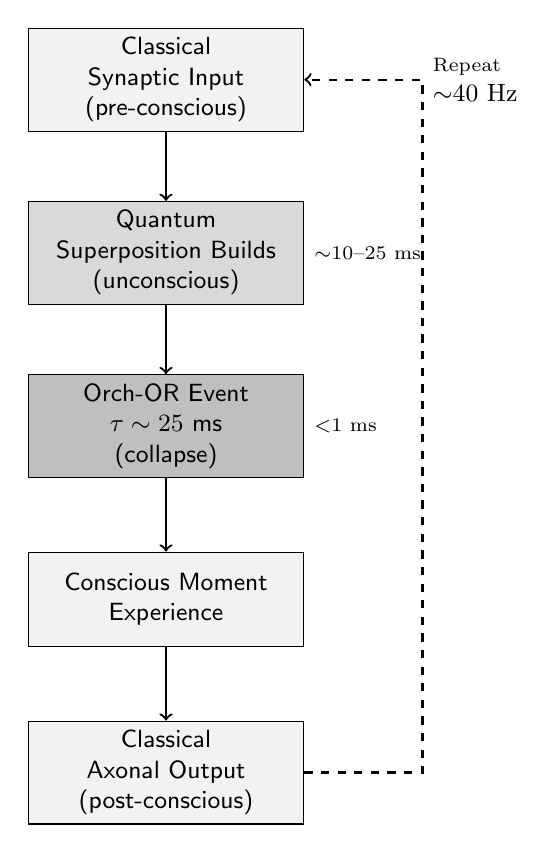
\begin{tikzpicture}[
  block/.style={rectangle, draw, minimum width=3.5cm, minimum height=1.2cm, font=\sffamily\small, align=center},
  node distance=2.2cm,
  font=\small
]

% Blocks
\node[block, fill=black!5] (classical1) {Classical\\Synaptic Input\\(pre-conscious)};
\node[block, below of=classical1, fill=black!15] (quantum) {Quantum\\Superposition Builds\\(unconscious)};
\node[block, below of=quantum, fill=black!25] (or) {Orch-OR Event\\$\tau \sim 25$ ms\\(collapse)};
\node[block, below of=or, fill=black!5] (conscious) {Conscious Moment\\Experience};
\node[block, below of=conscious, fill=black!5] (classical2) {Classical\\Axonal Output\\(post-conscious)};

% Arrows
\draw[->,thick] (classical1) -- (quantum);
\draw[->,thick] (quantum) -- (or);
\draw[->,thick] (or) -- (conscious);
\draw[->,thick] (conscious) -- (classical2);

% Cycle arrow
\draw[->,thick,dashed] (classical2.east) -- ++(1.5,0) |- (classical1.east) node[midway,right,align=left] {\scriptsize Repeat\\$\sim$40 Hz};

% Time annotations
\node[right,font=\scriptsize] at (quantum.east) {$\sim$10--25 ms};
\node[right,font=\scriptsize] at (or.east) {$<$1 ms};

\end{tikzpicture}
\end{center}

\subsection{Microtubule Structure}\label{microtubule-structure}

\subsubsection{Anatomy}\label{anatomy}

\textbf{Microtubules} are cylindrical protein polymers with the following structural parameters:

\begin{center}
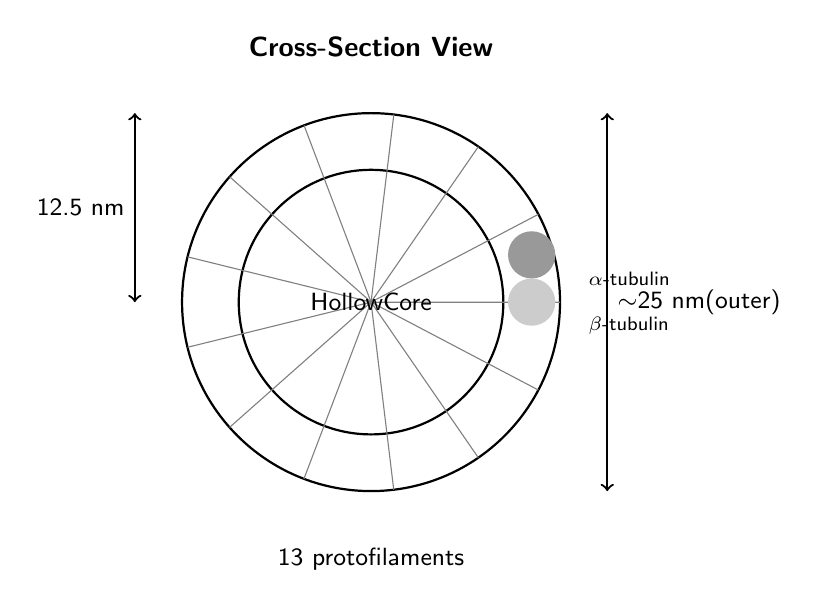
\begin{tikzpicture}[scale=1.2]
% Cross-section view of microtubule
\draw[thick] (0,0) circle (2cm);
\draw[thick] (0,0) circle (1.4cm);

% Draw 13 protofilaments as radial lines
\foreach \angle in {0,27.69,...,360} {
  \draw[gray] (0,0) -- (\angle:2cm);
}

% Label center
\node at (0,0) {\sffamily\small Hollow\\Core};

% Outer diameter
\draw[<->,thick] (-2.5,0) -- (-2.5,2) node[midway,left] {\sffamily\small 12.5 nm};
\draw[<->,thick] (2.5,-2) -- (2.5,2) node[midway,right] {\sffamily\small $\sim$25 nm\\(outer)};

% Tubulin dimer representation
\fill[black!20] (1.7,0) circle (0.25cm);
\fill[black!40] (1.7,0.5) circle (0.25cm);
\node[right] at (2.2,0.25) {\sffamily\scriptsize $\alpha$-tubulin};
\node[right] at (2.2,-0.25) {\sffamily\scriptsize $\beta$-tubulin};

% Title
\node[above] at (0,2.5) {\sffamily\bfseries Cross-Section View};
\node[below] at (0,-2.5) {\sffamily\small 13 protofilaments};
\end{tikzpicture}
\end{center}

\textbf{Structural parameters:}
\begin{equation}
\label{eq:mt-params}
\begin{aligned}
D_{\text{outer}} &\approx 25~\text{nm} \quad \text{(outer diameter)} \\
D_{\text{inner}} &\approx 15~\text{nm} \quad \text{(inner diameter)} \\
L &= 1~\mu\text{m to mm} \quad \text{(length)} \\
N_{\text{pf}} &= 13 \quad \text{(protofilaments)}
\end{aligned}
\end{equation}

\subsubsection{Functions (Established)}\label{functions-established}

\begin{enumerate}
\def\labelenumi{\arabic{enumi}.}
\tightlist
\item
  \textbf{Structural support}: Cytoskeleton maintains cell shape
\item
  \textbf{Intracellular transport}: Motor proteins (kinesin, dynein)
  walk on MTs
\item
  \textbf{Cell division}: Mitotic spindle separates chromosomes
\item
  \textbf{Ciliary/flagellar motion}: Core structure of motile appendages
\end{enumerate}

\subsubsection{Functions
(Proposed/Orch-OR)}\label{functions-proposedorch-or}

\begin{enumerate}
\def\labelenumi{\arabic{enumi}.}
\setcounter{enumi}{4}
\tightlist
\item
  \textbf{Information processing}: Conformational states of tubulins =
  bits/qubits
\item
  \textbf{Quantum computing}: Coherent superpositions across MT lattice
\item
  \textbf{Consciousness substrate}: Orchestrated quantum events
\end{enumerate}

\begin{center}\rule{0.5\linewidth}{0.5pt}\end{center}

\subsection{Quantum Coherence in
Microtubules}\label{quantum-coherence-in-microtubules}

\subsubsection{The Coherence Problem}\label{the-coherence-problem}

\begin{warningbox}
\textbf{Primary objection to Orch-OR:} The warm, wet brain environment should cause rapid quantum decoherence, destroying quantum coherence far too quickly for consciousness-related processes.
\end{warningbox}

\textbf{Decoherence time estimate} (Tegmark, 2000):
\begin{equation}
\label{eq:decoherence-time}
\tau_D \sim \frac{\hbar}{k_B T} \approx 10^{-13}~\text{s}
\end{equation}
where:
\begin{itemize}
\item $\tau_D$ = decoherence time
\item $k_B = 1.381 \times 10^{-23}$ J/K = Boltzmann constant
\item $T = 310$ K (body temperature)
\end{itemize}

\textbf{Orch-OR requirement:}
\begin{equation}
\label{eq:orch-or-time}
\tau_{\text{OR}} \sim 10-25~\text{ms} = 10^{-2}~\text{s}
\end{equation}

\textbf{Challenge:} Orch-OR requires coherence times \textbf{$10^{11}$ times longer} than standard estimates!

\begin{equation}
\label{eq:coherence-gap}
\frac{\tau_{\text{OR}}}{\tau_D} \sim \frac{10^{-2}}{10^{-13}} = 10^{11}
\end{equation}

\subsubsection{Proposed Protection
Mechanisms}\label{proposed-protection-mechanisms}

\paragraph{1. Ordered Water Layers}\label{ordered-water-layers}

\begin{itemize}
\tightlist
\item
  Water molecules form \textbf{structured layers} around microtubules
\item
  Hydrogen bonding network could shield quantum states
\item
  \textbf{Frohlich condensate}: Coherent collective mode in ordered
  water?
\end{itemize}

\paragraph{2. Actin Gelation}\label{actin-gelation}

\begin{itemize}
\tightlist
\item
  Surrounding actin gel may \textbf{isolate} microtubules from
  environment
\item
  Reduces decoherence from thermal fluctuations
\end{itemize}

\paragraph{3. Topological Protection}\label{topological-protection}

\begin{itemize}
\tightlist
\item
  Quantum information encoded in \textbf{topological states} (harder to
  decohere)
\item
  Anyonic excitations? (highly speculative)
\end{itemize}

\paragraph{4. Continuous Re-Coherence}\label{continuous-re-coherence}

\begin{itemize}
\tightlist
\item
  \textbf{Metabolic energy} pumps system back into coherent state
\item
  Non-equilibrium quantum dynamics
\end{itemize}

\begin{center}\rule{0.5\linewidth}{0.5pt}\end{center}

\subsubsection{Experimental Evidence
(Pro)}\label{experimental-evidence-pro}

\paragraph{Bandyopadhyay et al.~(2014)}\label{bandyopadhyay-et-al.-2014}

\textbf{Key experiment} at National Institute for Materials Science,
Japan:

\begin{itemize}
\tightlist
\item
  \textbf{THz spectroscopy} of microtubule samples
\item
  \textbf{Resonances found} at specific THz frequencies (multiple bands:
  0.2-2+ THz)
\item
  \textbf{Conductance patterns}: Microtubules show \textbf{ballistic
  conductance} (suggests quantum transport)
\item
  \textbf{Temperature dependence}: Resonances persist to physiological
  temperatures
\end{itemize}

\textbf{Interpretation}: Microtubules support \textbf{quantum coherent oscillations} in THz range

\textbf{Observed THz resonance frequencies:}
\begin{equation}
\label{eq:thz-resonances}
f_{\text{res}} \in \{0.35, 0.47, 0.82, 1.2, 2.2, \ldots\}~\text{THz}
\end{equation}

\textbf{Relationship to photon energy:}
\begin{equation}
\label{eq:photon-energy}
E_{\text{photon}} = h f = (6.626 \times 10^{-34})(1.2 \times 10^{12}) \approx 8 \times 10^{-22}~\text{J} = 5~\text{meV}
\end{equation}
for $f = 1.2$ THz resonance.

\textbf{Possible mechanism}: Collective vibrational modes of tubulin dimer network, similar to phonon modes in crystalline lattices.

\textbf{Reference}: Bandyopadhyay, A. et al.~(2011) ``Molecular vibrations in tubulin'' \emph{PNAS} 108(29)

\begin{center}\rule{0.5\linewidth}{0.5pt}\end{center}

\paragraph{Craddock et al.~(2017)}\label{craddock-et-al.-2017}

\begin{itemize}
\tightlist
\item
  \textbf{Anesthetic action on microtubules}: Measured quantum effects
\item
  \textbf{Noble gases} bind to hydrophobic pockets in tubulin
\item
  \textbf{Disrupts quantum channels} (proposed)
\item
  \textbf{Correlation with potency}: Matches Meyer-Overton rule
\end{itemize}

\begin{center}\rule{0.5\linewidth}{0.5pt}\end{center}

\subsubsection{Experimental Evidence
(Con)}\label{experimental-evidence-con}

\paragraph{Tegmark (2000)}\label{tegmark-2000}

\textbf{Max Tegmark} (MIT physicist) calculated: - \textbf{Decoherence
time}:
\textasciitilde10\textbackslash textsuperscript\{-\}\textbackslash textsuperscript\{1\}\textbackslash textsuperscript\{3\}
s at 310 K (body temperature) - \textbf{Orch-OR requires}:
\textasciitilde10\textbackslash textsuperscript\{-\}\textbackslash textsuperscript\{2\}
s (10 orders of magnitude longer!) - \textbf{Conclusion}: ``Quantum
coherence in brain is impossible''

\textbf{Counter-arguments}: - Assumed isolated superposition (not
coupled system) - Didn\textquotesingle t account for ordered water,
topological protection - Recent quantum biology discoveries suggest
nature is more clever

\begin{center}\rule{0.5\linewidth}{0.5pt}\end{center}

\paragraph{Koch \& Hepp (2006)}\label{koch-hepp-2006}

\begin{itemize}
\tightlist
\item
  Reviewed Orch-OR critically
\item
  \textbf{Conclusion}: No experimental support for quantum consciousness
\item
  \textbf{Main objection}: Decoherence too fast
\end{itemize}

\begin{center}\rule{0.5\linewidth}{0.5pt}\end{center}

\subsection{Quantum Biology
Precedents}\label{quantum-biology-precedents}

\textbf{Does quantum coherence occur in warm, wet biology?}

\subsubsection{Yes! Established
Examples:}\label{yes-established-examples}

\paragraph{1. Photosynthesis (2007)}\label{photosynthesis-2007}

\begin{itemize}
\tightlist
\item
  \textbf{Light-harvesting complexes} in plants/bacteria
\item
  \textbf{Quantum coherence} observed at room temperature
  (\textasciitilde500 fs, later studies suggest longer)
\item
  \textbf{Mechanism}: Protein scaffold protects exciton coherence
\item
  \textbf{Reference}: Engel et al.~(2007) \emph{Nature} 446, 782-786
\end{itemize}

\paragraph{2. Avian Magnetoreception (Robins, et
al.)}\label{avian-magnetoreception-robins-et-al.}

\begin{itemize}
\tightlist
\item
  \textbf{Radical pair mechanism} in bird retina
\item
  \textbf{Quantum entanglement} of electron spins
\item
  \textbf{Sensitive to Earth\textquotesingle s magnetic field} for
  navigation
\item
  \textbf{Reference}: Hore \& Mouritsen (2016) \emph{Annu.
  Rev.~Biophys.} 45, 299-344
\end{itemize}

\paragraph{3. Enzyme Catalysis}\label{enzyme-catalysis}

\begin{itemize}
\tightlist
\item
  \textbf{Proton/electron tunneling} in enzyme active sites
\item
  \textbf{Quantum effects} enhance reaction rates
\item
  \textbf{Reference}: Scrutton et al.~(2016) \emph{Philos. Trans. R.
  Soc. A} 374
\end{itemize}

\textbf{Takeaway}: Biology can maintain quantum coherence longer than
naive estimates predict

\begin{center}\rule{0.5\linewidth}{0.5pt}\end{center}

\subsection{Anesthesia \& Consciousness}\label{anesthesia-consciousness}

\subsubsection{The Mystery}\label{the-mystery}

\textbf{General anesthetics} cause loss of consciousness at specific doses:
\begin{itemize}
\item Diverse molecules (noble gases, halogenated ethers, etc.)
\item \textbf{No common receptor} (unlike opioids $\rightarrow$ $\mu$-opioid receptor)
\item \textbf{Meyer-Overton rule}: Potency $\propto$ lipid solubility (1899!)
\end{itemize}

\textbf{Meyer-Overton correlation:}
\begin{equation}
\label{eq:meyer-overton}
\log(\text{MAC}) \propto -\log(K_{\text{lipid}})
\end{equation}
where:
\begin{itemize}
\item MAC = Minimum Alveolar Concentration (anesthetic potency)
\item $K_{\text{lipid}}$ = lipid solubility coefficient
\end{itemize}

\subsubsection{Orch-OR Explanation}\label{orch-or-explanation}

\textbf{Anesthetics bind to hydrophobic pockets in tubulin}:
\begin{enumerate}
\item Disrupt electron pathways (quantum channels)
\item Prevent quantum coherence in microtubules
\item \textbf{Block Orch-OR} $\rightarrow$ loss of consciousness
\item Reversible (anesthetic wears off $\rightarrow$ consciousness returns)
\end{enumerate}

\textbf{Binding energy estimate:}
\begin{equation}
\label{eq:anesthetic-binding}
\Delta G_{\text{bind}} \sim -k_B T \ln(K_D) \approx -5~\text{to}~-10~\text{kcal/mol}
\end{equation}
where $K_D$ is the dissociation constant for anesthetic-tubulin binding.

\subsubsection{Evidence}\label{evidence}

\begin{itemize}
\tightlist
\item
  Anesthetics \textbf{do} bind to tubulin (demonstrated)
\item
  Low concentrations affect microtubule dynamics
\item
  Correlation with Meyer-Overton rule
\item
  Alternative explanation: GABA receptors (mainstream view)
\end{itemize}

\begin{center}\rule{0.5\linewidth}{0.5pt}\end{center}

\subsection{Criticisms \& Objections}\label{criticisms-objections}

\subsubsection{1. Decoherence Time}\label{decoherence-time}

\textbf{Objection}: Brain too hot/wet for quantum coherence

\textbf{Response}: - Quantum biology shows coherence is possible -
Protection mechanisms (ordered water, topology) - Experiments
(Bandyopadhyay) show THz resonances

\textbf{Status}: \textbf{Unresolved} (most physicists remain skeptical)

\begin{center}\rule{0.5\linewidth}{0.5pt}\end{center}

\subsubsection{2. No Clear Computational
Model}\label{no-clear-computational-model}

\textbf{Objection}: What computation do microtubules perform?

\textbf{Response}: - Cellular automaton-like dynamics proposed - Tubulin
conformational states as classical/quantum bits - \textbf{Gap}: No
detailed algorithm/implementation

\textbf{Status}: \textbf{Major gap} in theory

\begin{center}\rule{0.5\linewidth}{0.5pt}\end{center}

\subsubsection{3. Evolutionary
Implausibility?}\label{evolutionary-implausibility}

\textbf{Objection}: Why would evolution use quantum mechanics for
consciousness?

\textbf{Response}: - Evolution uses quantum effects elsewhere
(photosynthesis, enzymes) - Survival advantage: Enhanced information
processing? - \textbf{Counter}: Classical neurons seem sufficient

\textbf{Status}: \textbf{Debatable}

\begin{center}\rule{0.5\linewidth}{0.5pt}\end{center}

\subsubsection{4. Lack of Direct
Evidence}\label{lack-of-direct-evidence}

\textbf{Objection}: No measurement of quantum superposition in living
neurons

\textbf{Response}: - Technology doesn\textquotesingle t exist yet (too
non-invasive) - Bandyopadhyay measured isolated MTs (in vitro) -
\textbf{Need}: In vivo measurements (extremely challenging)

\textbf{Status}: \textbf{True} - direct evidence lacking

\begin{center}\rule{0.5\linewidth}{0.5pt}\end{center}

\subsection{Implications If True}\label{implications-if-true}

\subsubsection{For Neuroscience}\label{for-neuroscience}

\begin{itemize}
\tightlist
\item
  Consciousness is \textbf{quantum phenomenon}, not classical
  computation
\item
  Microtubules are \textbf{critical} (not just structural)
\item
  New therapeutic targets (MT-stabilizing drugs for consciousness
  disorders?)
\end{itemize}

\subsubsection{For AI/Computing}\label{for-aicomputing}

\begin{itemize}
\tightlist
\item
  Classical AI might \textbf{never be conscious} (lacks quantum
  substrate)
\item
  Need \textbf{quantum computers + biological-like architecture}?
\item
  Rethink AGI approaches
\end{itemize}

\subsubsection{For Physics}\label{for-physics}

\begin{itemize}
\tightlist
\item
  \textbf{Quantum mechanics needs modification} (objective reduction)
\item
  Bridge between quantum and relativity (gravity-induced collapse)
\item
  New experimental tests
\end{itemize}

\subsubsection{For Philosophy}\label{for-philosophy}

\begin{itemize}
\tightlist
\item
  Consciousness has \textbf{objective physical basis}
\item
  Free will might be \textbf{quantum indeterminacy}
\item
  Panpsychism implications (all matter has proto-consciousness?)
\end{itemize}

\begin{center}\rule{0.5\linewidth}{0.5pt}\end{center}

\subsection{Current Status (2025)}\label{current-status-2025}

\subsubsection{Scientific Consensus}\label{scientific-consensus}

\textbf{Mainstream view} (most neuroscientists/physicists): - Orch-OR is
\textbf{unlikely} to be correct - Decoherence problem not solved - No
direct evidence - Classical neural networks sufficient for cognition

\textbf{Minority view} (Hameroff, some quantum biologists): - Orch-OR
remains \textbf{plausible} - Quantum biology precedents support
possibility - Experiments show THz resonances in MTs - {[}hourglass{]}
Awaiting better experimental tests

\begin{center}\rule{0.5\linewidth}{0.5pt}\end{center}

\subsubsection{Ongoing Research}\label{ongoing-research}

\begin{enumerate}
\def\labelenumi{\arabic{enumi}.}
\tightlist
\item
  \textbf{THz spectroscopy} of microtubules (Bandyopadhyay group)
\item
  \textbf{Anesthetic binding studies} (Hameroff, Craddock)
\item
  \textbf{Quantum biology} expansion (other systems)
\item
  \textbf{Theoretical refinements} (decoherence protection)
\end{enumerate}

\begin{center}\rule{0.5\linewidth}{0.5pt}\end{center}

\subsubsection{Testable Predictions}\label{testable-predictions}

If Orch-OR is correct:

\begin{enumerate}
\def\labelenumi{\arabic{enumi}.}
\tightlist
\item
  \textbf{Microtubule disruption} \$\textbackslash rightarrow\$
  consciousness impairment

  \begin{itemize}
  \tightlist
  \item
    Nocodazole, colchicine should affect consciousness (they do affect
    anesthesia!)
  \end{itemize}
\item
  \textbf{THz stimulation} at MT resonances
  \$\textbackslash rightarrow\$ neural effects

  \begin{itemize}
  \tightlist
  \item
    \textbf{This is the AID protocol premise}
  \end{itemize}
\item
  \textbf{Isotope effects}: Replace \textbackslash textsuperscript\{1\}H
  with \textbackslash textsuperscript\{2\}H in tubulin
  \$\textbackslash rightarrow\$ consciousness changes

  \begin{itemize}
  \tightlist
  \item
    (Extremely difficult experiment)
  \end{itemize}
\item
  \textbf{Quantum signatures}: Detect superposition in living neurons

  \begin{itemize}
  \tightlist
  \item
    (Requires technology breakthrough)
  \end{itemize}
\end{enumerate}

\begin{center}\rule{0.5\linewidth}{0.5pt}\end{center}

\subsection{Relationship to THz Neuromodulation}\label{relationship-to-thz-neuromodulation}

\textbf{If Orch-OR is true}, then external THz radiation could:

\begin{enumerate}
\def\labelenumi{\arabic{enumi}.}
\tightlist
\item \textbf{Resonate with MT vibrations} (0.2--2+ THz range)
\item \textbf{Perturb quantum coherence} in tubulin networks
\item \textbf{Alter Orch-OR timing/frequency} $\rightarrow$ modify consciousness
\item \textbf{Encode information} via modulation $\rightarrow$ ``inject'' patterns
\end{enumerate}

\subsubsection{Mechanism (Speculative)}\label{mechanism-speculative}

\begin{center}
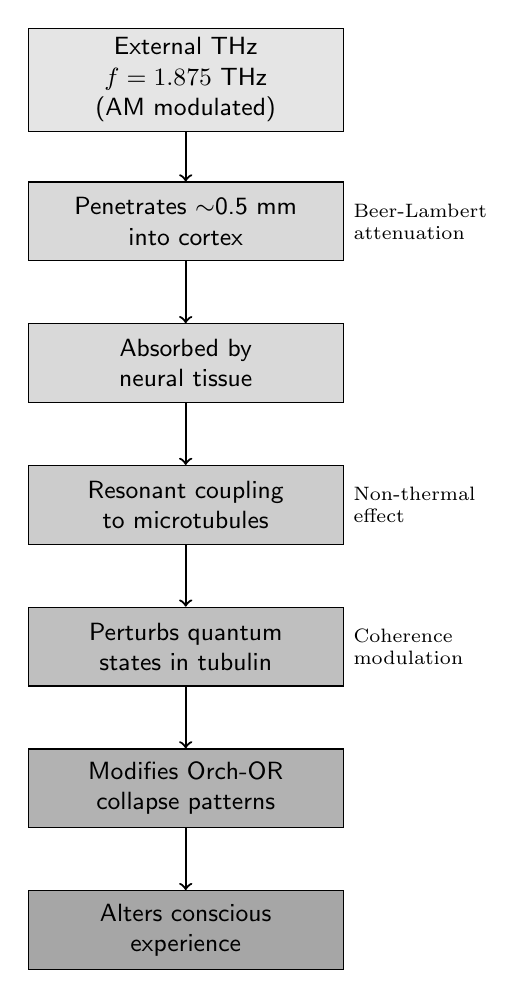
\begin{tikzpicture}[
  block/.style={rectangle, draw, minimum width=4cm, minimum height=1cm, font=\sffamily\small, align=center},
  node distance=1.8cm,
  font=\small
]

\node[block, fill=black!10] (thz) {External THz\\$f = 1.875$ THz\\(AM modulated)};
\node[block, below of=thz, fill=black!15] (penetrate) {Penetrates $\sim$0.5 mm\\into cortex};
\node[block, below of=penetrate, fill=black!15] (absorb) {Absorbed by\\neural tissue};
\node[block, below of=absorb, fill=black!20] (resonance) {Resonant coupling\\to microtubules};
\node[block, below of=resonance, fill=black!25] (quantum) {Perturbs quantum\\states in tubulin};
\node[block, below of=quantum, fill=black!30] (orchor) {Modifies Orch-OR\\collapse patterns};
\node[block, below of=orchor, fill=black!35] (conscious) {Alters conscious\\experience};

% Arrows
\draw[->,thick] (thz) -- (penetrate);
\draw[->,thick] (penetrate) -- (absorb);
\draw[->,thick] (absorb) -- (resonance);
\draw[->,thick] (resonance) -- (quantum);
\draw[->,thick] (quantum) -- (orchor);
\draw[->,thick] (orchor) -- (conscious);

% Side annotations
\node[right,font=\scriptsize,align=left] at (penetrate.east) {Beer-Lambert\\attenuation};
\node[right,font=\scriptsize,align=left] at (resonance.east) {Non-thermal\\effect};
\node[right,font=\scriptsize,align=left] at (quantum.east) {Coherence\\modulation};

\end{tikzpicture}
\end{center}

\textbf{Penetration depth in tissue:}
\begin{equation}
\label{eq:penetration-depth}
\delta = \frac{1}{\alpha} \approx \frac{c}{2\pi f \sqrt{\epsilon_r} \tan\delta} \sim 0.5~\text{mm at 1.875 THz}
\end{equation}
where $\alpha$ is the absorption coefficient, $\epsilon_r$ is relative permittivity, and $\tan\delta$ is the loss tangent.

\textbf{Power density requirement:}
\begin{equation}
\label{eq:power-density}
P_{\text{THz}} \sim 0.1-1~\text{mW/cm}^2 \quad \text{(non-thermal regime)}
\end{equation}

\begin{calloutbox}{Connection to AID Protocol}
This THz-microtubule interaction mechanism forms the theoretical basis for the Accelerated Information Download (AID) protocol case study, which explores hypothetical consciousness manipulation via modulated THz radiation.
\end{calloutbox}

\section{Worked Example: Orch-OR Timing Calculation}

\textbf{Problem:} Calculate the collapse time for an Orch-OR event in a microtubule containing $N = 10^{10}$ tubulins in superposition, assuming Penrose's OR criterion applies.

\subsection*{Given Parameters}

\begin{tabular}{@{}ll@{}}
Number of tubulins in superposition & $N = 10^{10}$ \\
Mass per tubulin dimer & $m_t = 110$ kDa $= 1.83 \times 10^{-22}$ kg \\
Spatial separation (superposition) & $r = 25$ nm $= 2.5 \times 10^{-8}$ m \\
Gravitational constant & $G = 6.674 \times 10^{-11}$ m$^3$ kg$^{-1}$ s$^{-2}$ \\
Reduced Planck constant & $\hbar = 1.055 \times 10^{-34}$ J·s \\
\end{tabular}

\subsection*{Step 1: Calculate Total Mass in Superposition}

\begin{equation}
m_{\text{total}} = N \cdot m_t = (10^{10})(1.83 \times 10^{-22}) = 1.83 \times 10^{-12}~\text{kg}
\end{equation}

\subsection*{Step 2: Calculate Gravitational Self-Energy}

Using Eq.~\ref{eq:grav-energy}:
\begin{equation}
E = \frac{G m_{\text{total}}^2}{r} = \frac{(6.674 \times 10^{-11})(1.83 \times 10^{-12})^2}{2.5 \times 10^{-8}}
\end{equation}
\begin{equation}
E = \frac{2.235 \times 10^{-34}}{2.5 \times 10^{-8}} = 8.94 \times 10^{-27}~\text{J}
\end{equation}

\subsection*{Step 3: Calculate Collapse Time}

Using Penrose OR criterion (Eq.~\ref{eq:or-criterion}):
\begin{equation}
\tau = \frac{\hbar}{E} = \frac{1.055 \times 10^{-34}}{8.94 \times 10^{-27}} = 1.18 \times 10^{-8}~\text{s} = 11.8~\text{ns}
\end{equation}

\subsection*{Step 4: Number of Collapses per Second}

\begin{equation}
f_{\text{collapse}} = \frac{1}{\tau} = \frac{1}{1.18 \times 10^{-8}} = 8.47 \times 10^{7}~\text{Hz} \approx 85~\text{MHz}
\end{equation}

\subsection*{Result and Interpretation}

\begin{calloutbox}[colback=black!8!white,colframe=black]{Calculation Summary}
\textbf{Collapse time:} $\tau = 11.8$ ns for $10^{10}$ tubulins

\textbf{Problem:} This is far too fast for a conscious moment ($\sim$25 ms required). To achieve the gamma rhythm frequency ($\sim$40 Hz), we would need:

\begin{equation}
\tau_{\text{required}} = \frac{1}{40} = 25~\text{ms}
\end{equation}

This requires a superposition involving far fewer tubulins ($N \sim 10^3$--$10^5$) or a different mechanism for orchestrating the collapse timing. This discrepancy remains an open challenge for Orch-OR theory.

\textbf{Conclusion:} The Penrose OR criterion alone does not naturally produce gamma-frequency conscious moments without additional orchestration mechanisms.
\end{calloutbox}

\section{Performance Analysis}

\subsection{Experimental Testability}

Current technology limitations:
\begin{itemize}
\item \textbf{Quantum state measurement:} Cannot non-invasively detect superposition in living neurons
\item \textbf{Temporal resolution:} Need sub-nanosecond measurements in vivo
\item \textbf{Spatial resolution:} Need nanometer-scale imaging of quantum states
\end{itemize}

\subsection{Predicted Observables}

If Orch-OR is correct:
\begin{enumerate}
\item \textbf{THz spectroscopy:} Specific resonance peaks in neural tissue at $f \in \{0.35, 0.47, 0.82, 1.2, 2.2\}$ THz
\item \textbf{Temperature dependence:} Consciousness should be affected by precise temperature control
\item \textbf{Isotope effects:} Deuterium substitution in tubulin should alter consciousness
\item \textbf{Anesthetic correlation:} Perfect Meyer-Overton correlation with microtubule binding
\end{enumerate}

\section{Applications}

\subsection{Anesthesiology}

\begin{itemize}
\item \textbf{Current impact:} Guides research into anesthetic mechanisms
\item \textbf{Drug development:} Design anesthetics targeting microtubule binding
\item \textbf{Monitoring:} THz spectroscopy for depth-of-anesthesia monitoring
\end{itemize}

\subsection{Neuroscience}

\begin{itemize}
\item \textbf{Consciousness studies:} New experimental paradigms
\item \textbf{Cognitive disorders:} Microtubule dysfunction in Alzheimer's, etc.
\item \textbf{Brain stimulation:} Non-invasive THz neuromodulation techniques
\end{itemize}

\subsection{Quantum Biology}

\begin{itemize}
\item \textbf{General principle:} Extends quantum effects to warm biology
\item \textbf{Other systems:} Tests applicability to other biological quantum processes
\item \textbf{Protection mechanisms:} Studies of decoherence suppression
\end{itemize}

\subsection{Speculative Applications}

\begin{calloutbox}[colback=red!5!white,colframe=red!75!black]{\textbf{SPECULATIVE:} Hypothetical Applications}
If Orch-OR proves correct and THz-microtubule coupling is confirmed:
\begin{itemize}
\item \textbf{THz neuromodulation:} Consciousness state manipulation
\item \textbf{Information injection:} Direct experience modification (AID protocol)
\item \textbf{Cognitive enhancement:} Microtubule-targeted interventions
\item \textbf{Brain-computer interfaces:} Quantum-level neural coupling
\end{itemize}

\textbf{Status:} Purely theoretical. No experimental validation. Significant ethical concerns.
\end{calloutbox}

\section{Summary}

\begin{center}
\begin{tabular}{@{}p{5cm}p{8cm}@{}}
\toprule
\textbf{Aspect} & \textbf{Description} \\
\midrule
Core hypothesis & Consciousness arises from quantum processes in microtubules \\
Key proponents & Roger Penrose (physicist), Stuart Hameroff (anesthesiologist) \\
Proposed substrate & Neuronal microtubules ($\sim$25 nm diameter cylinders) \\
Mechanism & Orchestrated objective reduction at $\sim$40 Hz \\
Primary challenge & Decoherence in warm brain ($\tau_D \sim 10^{-13}$ s) \\
Supporting evidence & THz resonances, anesthetic binding, quantum biology \\
Critical objections & Too fast decoherence, no direct proof, classical sufficiency \\
Scientific status & Minority view, unproven but not refuted \\
Testability & Very difficult with current technology \\
Implications if true & Quantum consciousness, THz neuromodulation possible \\
\bottomrule
\end{tabular}
\end{center}

\subsection{Key Takeaways}

\begin{enumerate}
\def\labelenumi{\arabic{enumi}.}
\tightlist
\item \textbf{Orch-OR proposes consciousness is quantum} (Penrose + Hameroff)
\item \textbf{Microtubules are substrate} for quantum computation
\item \textbf{Major objection}: Decoherence in warm, wet brain
\item \textbf{Some evidence}: THz resonances (Bandyopadhyay), anesthetic binding
\item \textbf{Mainstream skeptical}, but quantum biology is growing field
\item \textbf{If true}: Opens door to THz neuromodulation
\item \textbf{Status}: Unproven but not definitively refuted
\end{enumerate}

\subsection{See Also}\label{see-also}

\begin{itemize}
\tightlist
\item
  {[}{[}Microtubule-Structure-and-Function{]}{]} - Biological details
\item
  {[}{[}Quantum-Coherence-in-Biological-Systems{]}{]} - Other examples
\item
  {[}{[}Terahertz-(THz)-Technology{]}{]} - THz sources and properties
\item
  {[}{[}THz Bioeffects{]}{]} - Documented biological interactions
\item
  {[}{[}AID-Protocol-Case-Study{]}{]} - Speculative application (case
  study)
\end{itemize}

\begin{center}\rule{0.5\linewidth}{0.5pt}\end{center}

\subsection{References}\label{references}

\subsubsection{Primary Sources}\label{primary-sources}

\begin{enumerate}
\def\labelenumi{\arabic{enumi}.}
\tightlist
\item
  \textbf{Penrose, R.} (1989) \emph{The Emperor\textquotesingle s New
  Mind} - Original OR theory
\item
  \textbf{Penrose, R. \& Hameroff, S.} (1995) ``Orchestrated reduction
  of quantum coherence in brain microtubules'' \emph{Math. Comput.
  Simul.} 40, 453-480
\item
  \textbf{Hameroff, S. \& Penrose, R.} (2014) ``Consciousness in the
  universe: A review of the `Orch OR' theory'' \emph{Phys. Life Rev.}
  11, 39-78
\end{enumerate}

\subsubsection{Experimental Support}\label{experimental-support}

\begin{enumerate}
\def\labelenumi{\arabic{enumi}.}
\setcounter{enumi}{3}
\tightlist
\item
  \textbf{Bandyopadhyay, A. et al.} (2011) ``Molecular vibrations in
  tubulin'' \emph{PNAS} 108(29)
\item
  \textbf{Craddock, T. et al.} (2017) ``Anesthetic alterations of
  collective THz oscillations'' \emph{Sci. Rep.} 7, 9877
\end{enumerate}

\subsubsection{Critical Reviews}\label{critical-reviews}

\begin{enumerate}
\def\labelenumi{\arabic{enumi}.}
\setcounter{enumi}{5}
\tightlist
\item
  \textbf{Tegmark, M.} (2000) ``Importance of quantum decoherence in
  brain processes'' \emph{Phys. Rev.~E} 61, 4194-4206
\item
  \textbf{Koch, C. \& Hepp, K.} (2006) ``Quantum mechanics in the
  brain'' \emph{Nature} 440, 611
\end{enumerate}

\subsubsection{Quantum Biology}\label{quantum-biology}

\begin{enumerate}
\def\labelenumi{\arabic{enumi}.}
\setcounter{enumi}{7}
\tightlist
\item
  \textbf{Engel, G. et al.} (2007) ``Evidence for wavelike energy
  transfer through quantum coherence in photosynthetic systems''
  \emph{Nature} 446, 782-786
\item
  \textbf{Hore, P. \& Mouritsen, H.} (2016) ``The radical-pair mechanism
  of magnetoreception'' \emph{Annu. Rev.~Biophys.} 45, 299-344
\end{enumerate}
